% Class option 't' makes elements preserve position when \only<n> is used
\documentclass[ignorenonframetext,t]{beamer}
      
% 2,4-10,14,17-44
% These geometries are all FHD (1920x1080), but they result in different
% font sizes.  Watch the titlepage!
%\geometry{papersize={19.2cm,10.80cm}}
%\geometry{papersize={11.52cm,6.48cm}}  % as above, but 3/5  (0.6)
\geometry{papersize={12.8cm,7.2cm}}	% as above, but 2/3  (0.66)
%\geometry{papersize={14.4cm,8.1cm}}	% as above, but 3/4  (0.75)


\setbeameroption{show notes}
% \usepackage[overridenote]{pdfpc} % BEWARE: changes note contents interpretation

\usepackage[spanish]{babel}
\usepackage[T1]{fontenc}
\usepackage[utf8]{inputenc}
\usepackage[export]{adjustbox} % https://texblog.org/2014/02/20/figure-with-border-in-latex/
\usepackage[normalem]{ulem}
\usepackage{relsize}

% make links blue
\hypersetup{
    colorlinks = true,
    urlcolor   = blue,
}

\let\checkmark\undefined  % dingbat defines this, but it's already been defined previously. wtf.
\usepackage{dingbat} % WARNING -- hacked up!

\usepackage{textcomp}	% for \textrightarrow

\usepackage{pgfpages}
%\setbeameroption{show notes}
%\setbeameroption{show notes on second screen=right}

% 19.5x9 is alvherre's current phone aspect ratio
%\geometry{papersize={19.5cm,9cm}}
\IfFileExists{upquote.sty}{\usepackage{upquote}}{}

\usetheme{Frankfurt}
\setbeamertemplate{items}[circle] 
\beamertemplatenavigationsymbolsempty

% Minimal changes to color palette, using EDB colors
\definecolor{bluecoal}{RGB}{40, 73, 90}
\definecolor{goldleaf}{RGB}{231,197,104}
\setbeamercolor{structure}{fg=bluecoal}
\setbeamercolor{palette primary}{fg=goldleaf}

% https://tex.stackexchange.com/questions/673635/beamer-section-title-slides
\setbeamertemplate{section page}
{
  \begingroup
    \centering
%    {\usebeamerfont{section name}\usebeamercolor[fg]{section name}\sectionname~\insertsectionnumber}
    \vskip1em\par
    \begin{beamercolorbox}[sep=12pt,center,rounded=true]{section title}
      \usebeamerfont{section title}\insertsection\par
    \end{beamercolorbox}
  \endgroup
}


% Definitions for title page
% Maybe define graphic sizes in terms of pagesize fractions?
\title{Table Repacking, done right}

\author{Antonín Houska -- Postgres developer, CYBERTEC \\
Álvaro Herrera -- Postgres developer, EDB}
\newcommand{\sizeforedblogo}{0.11}
\newcommand{\sizeforconflogo}{0.13}
\newcommand{\sizeforlogos}{0.1}
\newcommand{\sizeforimages}{0.8}
% \institute{\vspace*{-0.2cm}\href{https://www.enterprisedb.com/}{
\includegraphics[height=\sizeforlogos\paperheight]{edb_portrait_color_grey.png}} \hspace{1cm} \href{https://p2d2.cz/2025/}{
\includegraphics[height=\sizeforlogos\paperheight]{p2d2_logo_1.png}}}
\institute{\vspace*{-0.2cm}\href{https://www.enterprisedb.com/}{
\includegraphics[height=\sizeforedblogo\paperheight]{edb_postgres_ai.png}} \hspace{1cm} \href{https://2025.pgconf.eu/}{
\includegraphics[height=\sizeforconflogo\paperheight]{logo_pgconf_eu.jpg}} \hspace{1cm} \href{https://cybertec.at/}{
\includegraphics[height=\sizeforlogos\paperheight]{CYBERTEC-logo-without-claim.png}}}
\date{Postgres Conference Europe 2025 \\
Riga, Latvia \\
23-24 October 2025}

%\href{https://p2d2.cz/2025/}{
\includegraphics[width=2cm]{p2d2_logo_1.png}} \\

% Footer for all slides
\setbeamertemplate{footline}{%
  \hspace{0.3cm}%
  \href{https://www.enterprisedb.com/}{
\includegraphics[height=.45cm]{edb_postgres_ai_lightmode-100.jpg}}%
  \hfill%
  \href{https://2025.pgconf.eu/}{
\includegraphics[height=20px]{logo_pgconf_eu.jpg}}\hspace{0.3cm}%
  \hfill%
  \href{https://www.cybertec.at/}{
\includegraphics[height=.4cm]{CYBERTEC-logo-without-claim.png}}%
  \hspace{0.3cm}%
  }

%https://tex.stackexchange.com/questions/119277/non-bitmapped-thumb-up-symbol-for-flagging-good-practice-tips
\usepackage{fontawesome}

\usepackage{pmboxdraw}


% https://tex.stackexchange.com/questions/58922/beamer-using-pause-within-lstlisting
\usepackage{listings}
\lstset{language=SQL,
basicstyle=\footnotesize\ttfamily,keywordstyle=\bfseries\color{green!40!black},%
columns=fullflexible, keepspaces, upquote,
escapeinside={\%*}{*)},
morekeywords={with, merge, returning, repack},
deletekeywords={YEAR},
showspaces=false,showstringspaces=false,
literate={á}{{\'{a}}}{1}
         {é}{{\'{e}}}{1}
         {í}{{\'{i}}}{1}
         {ó}{{\'{o}}}{1}
         {ú}{{\'{u}}}{1}
         {ñ}{{\~{n}}}{1}
	 {°}{\textdegree}{1}
         {¡}{{!`}}{1}
         {┌}{{\textSFi}}1 
         {─}{{\textSFx}}1 
         {│}{{\pmboxdrawuni{2502}}}1
         {┬}{{\textSFvi}}1
         {┐}{{\textSFiii}}1
         {├}{{\textSFviii}}1
         {┼}{{\textSFv}}1
         {┤}{{\textSFix}}1
         {┴}{{\textSFvii}}1
         {└}{{\textSFii}}1
         {┘}{{\textSFiv}}1
	 {↵}{{\carriagereturn}}1
%morekeywords={data,wrapper,library,language}%
}

%\newcommand{\putcollection}{
%  \put(0,50){
%    \parbox{\textwidth}{
%      \fontsize{30}{30}\selectfont
%      Álvaro Herrera \\
%      PostgreSQL developer \\
%      EDB
%    }
%  }
%}
%\newcommand{\insertcopyright}{}
%\renewcommand{\insertcopyright}{
\includegraphics[height=10px]{topbarlogo-grey.png}\hspace{1cm}{}}
%\date{}

% Make pauses show greyed-out future text
\setbeamercovered{transparent}

% :vim:set sw=3:
\newcommand{\linksize}{\scriptsize}
%\newcommand{\textrightarrow}{$\,\to\,$}
\begin{document}

\begin{frame}[plain]
  \titlepage
\end{frame}


\begin{frame}
	\frametitle{Antonín Houska}
  \begin{itemize}
    \item Antonín Houska, \href{mailto:ah@cybertec.at}{ah@cybertec.at}
    \item Postgres contributor since 2012
    \item Working as a Postgres developer for CYBERTEC since 2012
  \end{itemize}
\end{frame}

\begin{frame}
	\frametitle{Álvaro Herrera}
  \begin{itemize}
    \item Álvaro Herrera, \href{mailto:alvherre@kurilemu.de}{alvherre@kurilemu.de}
    \item Postgres contributor since 2002
    \item Working as a Postgres developer for 2ndQuadrant/EDB since 2012
\begin{itemize} \item \linksize Feel free to grab hold of me on hallways to talk about stuff \end{itemize}
  \end{itemize}
\end{frame}

\begin{frame}
  \frametitle{Talk structure}
  \begin{enumerate}
    \item The problem: table bloat
    \item The historical solution: VACUUM FULL
    \item Third-party solutions
	    \begin{itemize}
		    \item \emph{pg\_repack}
		    \item \emph{pg\_squeeze}
	    \end{itemize}
    \item Non-concurrent REPACK
    \item REPACK CONCURRENTLY
  \end{enumerate}
\end{frame}

\section{Historical review}

\begin{frame}
	\frametitle{The problem: table bloat}
\end{frame}

\begin{frame}
	\frametitle{VACUUM FULL}
\end{frame}

\begin{frame}
	\frametitle{\texttt{pg\_repack}}
  \begin{itemize}
    \item Forked from \texttt{pg\_reorg} in 2012 (\texttt{pg\_reorg} started
      in 2008)
    \item SQL and C functions installed on server, but the workflow is
      controlled by a client application
    \item Like VACUUM FULL / CLUSTER it removes the bloat by copying the
      useful data to a new table, swaps the files and drops the new
      table. Exclusive lock is held only during the swap.
    \item Data changes done by applications during the copying are captured by
      triggers and written to a ``log table''. They are applied right before
      the swap.
  \end{itemize}
\end{frame}

\begin{frame}
  \frametitle{\texttt{pg\_repack}}
  \begin{center}
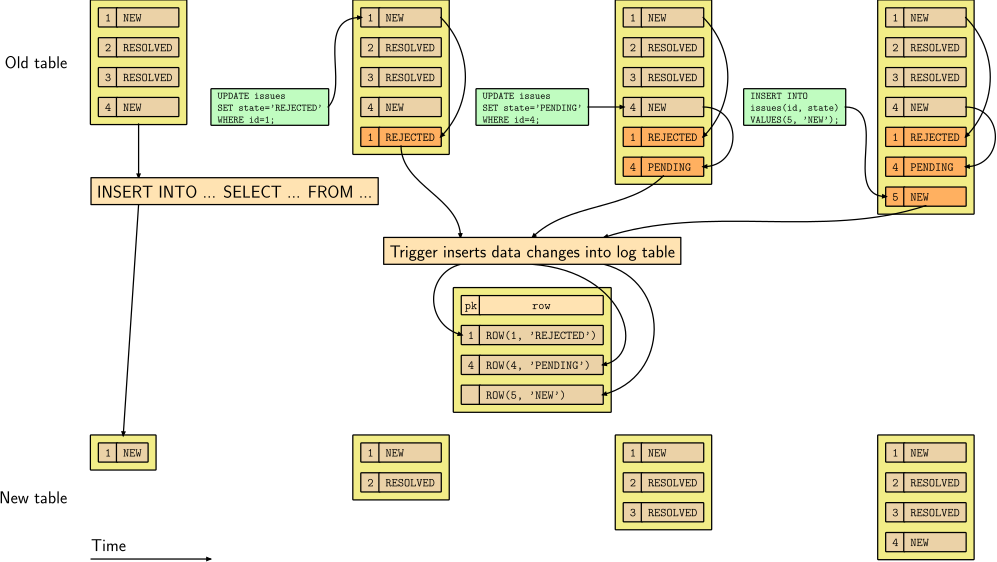
\includegraphics[height=\sizeforimages\textheight]{pg_repack_01.png}
  \end{center}
\end{frame}

\begin{frame}
  \frametitle{\texttt{pg\_repack}}
  \begin{center}
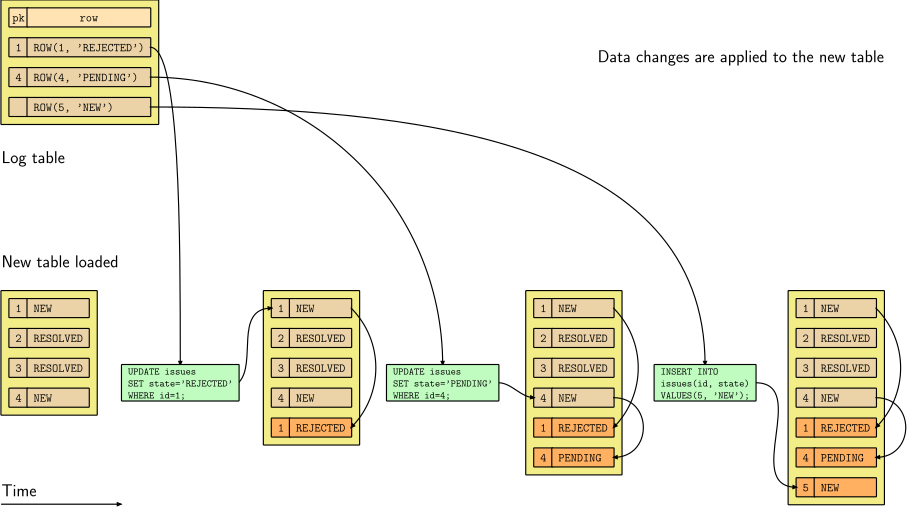
\includegraphics[height=\sizeforimages\textheight]{pg_repack_02.png}
  \end{center}
\end{frame}

\begin{frame}
        \frametitle{\texttt{pg\_squeeze}}
  \begin{itemize}
    \item Started in 2016 (PostgreSQL 9.5)
    \item The idea was to use background worker to launch \texttt{pg\_repack} automatically
    \item \texttt{pg\_repack} is implemented both on server and client side --
      not really suitable for background worker
    \item PostgreSQL 9.4 introduced logical decoding -- I thought it should be
      simpler to use this instead of triggers to capture data changes
    \item Use server API rather than SQL commands to manipulate tables,
      indexes and data.
  \end{itemize}
\end{frame}

\begin{frame}
  \frametitle{\texttt{pg\_squeeze}}
  \begin{center}
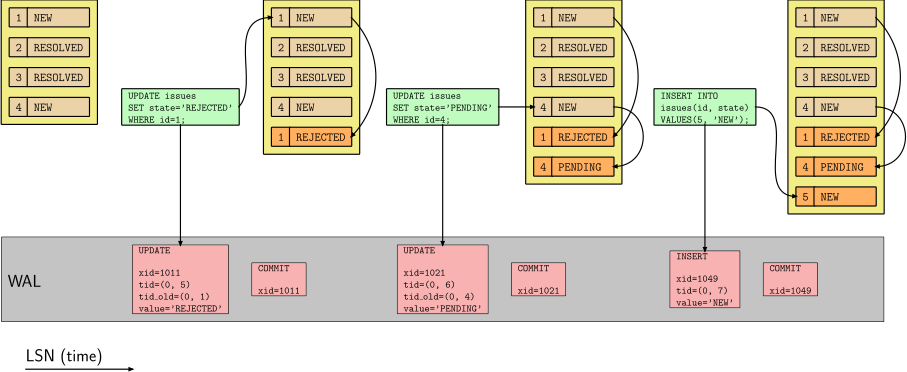
\includegraphics[height=\sizeforimages\textheight]{pg_squeeze_01.png}
  \end{center}
\end{frame}

\begin{frame}
  \frametitle{\texttt{pg\_squeeze}}
  \begin{center}
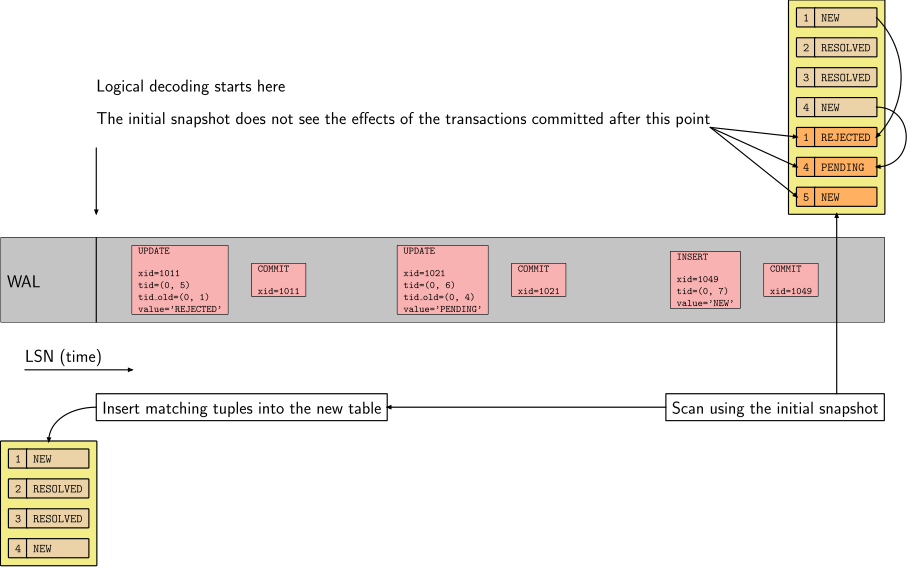
\includegraphics[height=\sizeforimages\textheight]{pg_squeeze_02.png}
  \end{center}
\end{frame}

\begin{frame}
  \frametitle{\texttt{pg\_squeeze}}
  \begin{center}
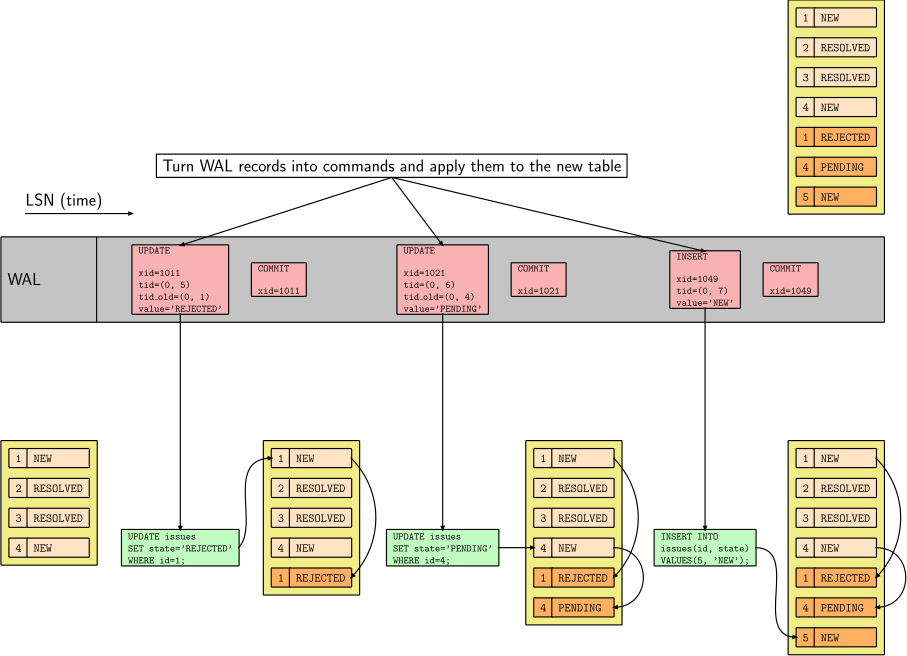
\includegraphics[height=\sizeforimages\textheight]{pg_squeeze_03.png}
  \end{center}
\end{frame}

\begin{frame}
        \frametitle{\texttt{pg\_squeeze}}
%% TODO 1. Disk space requirements, 2. Scheduling, 3. GUC for maximum lock time
%% (probably not used much)
\end{frame}


\section{Repacking done right}
\begin{frame}
	\frametitle{The REPACK command}
\end{frame}

\subsection{Concurrent Repacking}
\begin{frame}
	\frametitle{REPACK CONCURRENTLY}

% TODO (if there's enough time) Explain differences between pg_squeeze and
% REPACK CONCURRENTLY.
%
% 1. pg_squeeze uses AccessShareLock and releases it before it requests
% AccessExclusiveLock (for the file swap), in order to avoid deadlock. If the
% table changed in between, the whole processing is aborted. This approach is
% proably overly cautious. In REPACK CONCURRENTLY, we use
% ShareUpdateExclusiveLock and then simply upgrade it to AccessExclusiveLock,
% so we don't have to check for concurrent catalog changes. (The risk of
% deadlock during the lock upgrade is probably low.)
%
% 2. Since REPACK CONCURRENTLY does not release the ShareUpdateExclusiveLock
% until done, and since this lock conflicts with VACUUM, it does not have to
% care about the xmin horizon (Note: setting the slot's xmin to
% InvalidTransactionId is yet to be implemented.) On the other hand,
% pg_squeeze allows for VACUUM most of the time, so has to block the xmin
% horizon until the initial copy is complete.
%
% 2. Unlike extension, the core code can implement MVCC safety. (Although not
% necessarily in PG 19).
%
% 3. REPACK does not implement scheduling - not sure it's necessary,
% extensions can do that.
\end{frame}


\section{Future work}
\begin{frame}
  \frametitle{Future work}
  %% TODO 1. Logical decoding by background worker, 2. MVCC safety.
\end{frame}


\begin{frame}
  \frametitle{Thanks for listening!}
  \vfill
  \begin{columns}[T]
    \begin{column}{0.6\textwidth}
      { \LARGE Questions? }

      \begin{center}
	\vspace{0.3cm}
	Antonín Houska, {\color{bluecoal}  \href{https://cybertec.at/}{CYBERTEC}} \\
	\href{mailto:ah@cybertec.at}{\texttt{ah@cybertec.at}} \\
	\vspace{0.5cm}
	Álvaro Herrera, {\color{bluecoal}  \href{https://enterprisedb.com/}{EDB}} \\
	\href{mailto:alvherre@kurilemu.de}{\texttt{alvherre@kurilemu.de}}
      \end{center}
    \end{column}
    \begin{column}{0.25\textwidth}
      
\includegraphics[height=0.7\textwidth]{qr-repack.png}
      \raggedleft{Leave Feedback!}
    \end{column}
  \end{columns}
  \vfill
\end{frame}


\end{document}

% :vim:ts=4:sw=4
